\documentclass{standalone}
\usepackage{tikz}
\usetikzlibrary{patterns, positioning}


\begin{document}
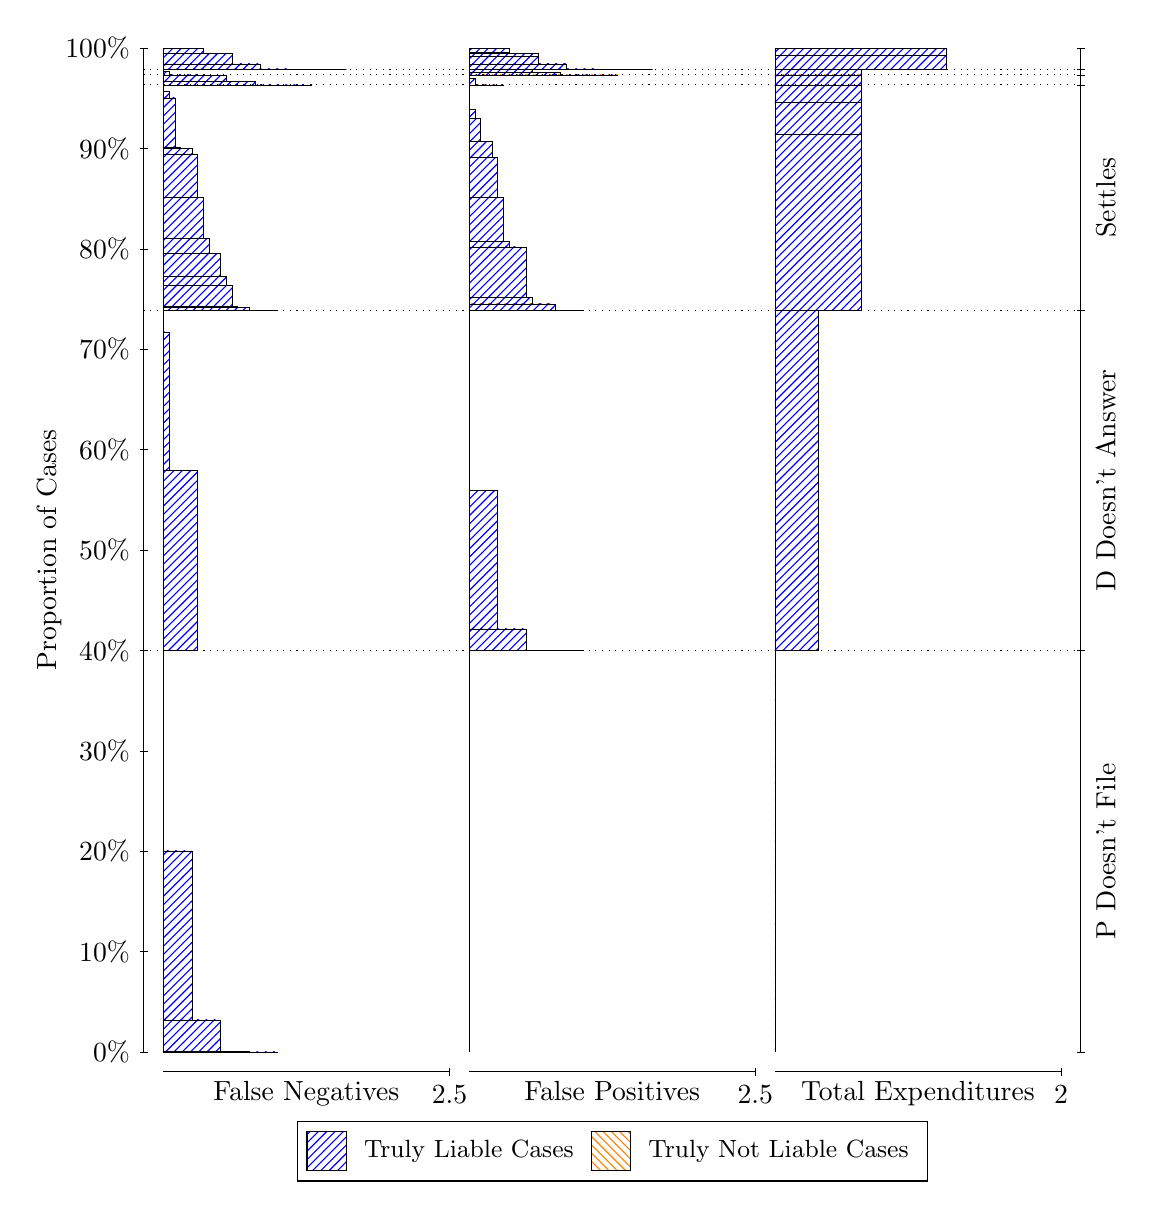
\begin{tikzpicture}
\draw[black, very thin] (1.5,1.75) -- (1.5,14.5);
\node[rotate=90, text=black, anchor=center] at (0.3, 8.125) {Proportion of Cases};
\draw[black, very thin] (1.45,1.75) -- (1.55,1.75);
\node[text=black, anchor=east] at (1.45, 1.75) {0\%};
\draw[black, very thin] (1.45,3.025) -- (1.55,3.025);
\node[text=black, anchor=east] at (1.45, 3.025) {10\%};
\draw[black, very thin] (1.45,4.3) -- (1.55,4.3);
\node[text=black, anchor=east] at (1.45, 4.3) {20\%};
\draw[black, very thin] (1.45,5.575) -- (1.55,5.575);
\node[text=black, anchor=east] at (1.45, 5.575) {30\%};
\draw[black, very thin] (1.45,6.85) -- (1.55,6.85);
\node[text=black, anchor=east] at (1.45, 6.85) {40\%};
\draw[black, very thin] (1.45,8.125) -- (1.55,8.125);
\node[text=black, anchor=east] at (1.45, 8.125) {50\%};
\draw[black, very thin] (1.45,9.4) -- (1.55,9.4);
\node[text=black, anchor=east] at (1.45, 9.4) {60\%};
\draw[black, very thin] (1.45,10.675) -- (1.55,10.675);
\node[text=black, anchor=east] at (1.45, 10.675) {70\%};
\draw[black, very thin] (1.45,11.95) -- (1.55,11.95);
\node[text=black, anchor=east] at (1.45, 11.95) {80\%};
\draw[black, very thin] (1.45,13.225) -- (1.55,13.225);
\node[text=black, anchor=east] at (1.45, 13.225) {90\%};
\draw[black, very thin] (1.45,14.5) -- (1.55,14.5);
\node[text=black, anchor=east] at (1.45, 14.5) {100\%};

\draw[black, very thin] (13.4,1.75) -- (13.4,14.5);
\draw[black, very thin] (13.35,1.75) -- (13.45,1.75);
\node[anchor=west] at (13.35, 1.75) {};
\draw[black, very thin] (13.35,6.8489) -- (13.45,6.8489);
\node[anchor=west] at (13.35, 6.8489) {};
\draw[black, very thin] (13.35,11.17) -- (13.45,11.17);
\node[anchor=west] at (13.35, 11.17) {};
\draw[black, very thin] (13.35,14.032) -- (13.45,14.032);
\node[anchor=west] at (13.35, 14.032) {};
\draw[black, very thin] (13.35,14.159) -- (13.45,14.159);
\node[anchor=west] at (13.35, 14.159) {};
\draw[black, very thin] (13.35,14.231) -- (13.45,14.231);
\node[anchor=west] at (13.35, 14.231) {};
\draw[black, very thin] (13.35,14.5) -- (13.45,14.5);
\node[anchor=west] at (13.35, 14.5) {};

\draw[black, very thin, pattern color=blue, pattern=north east lines] (1.75,1.75) rectangle (3.2033,1.75);
\draw[black, very thin, pattern color=blue, pattern=north east lines] (1.75,1.75) rectangle (2.84,1.7534);
\draw[black, very thin, pattern color=blue, pattern=north east lines] (1.75,1.7534) rectangle (2.4767,2.158);
\draw[black, very thin, pattern color=blue, pattern=north east lines] (1.75,2.158) rectangle (2.1133,4.3029);
\draw[black, very thin, pattern color=orange, pattern=north west lines] (1.75,4.3029) rectangle (1.75,4.3029);
\draw[black, very thin, pattern color=blue, pattern=north east lines] (1.75,4.3029) rectangle (1.75,6.8489);
\draw[black, very thin, pattern color=blue, pattern=north east lines] (1.75,6.8489) rectangle (2.186,9.1329);
\draw[black, very thin, pattern color=blue, pattern=north east lines] (1.75,9.1329) rectangle (1.8227,10.896);
\draw[black, very thin, pattern color=orange, pattern=north west lines] (1.75,10.896) rectangle (1.75,10.896);
\draw[black, very thin, pattern color=blue, pattern=north east lines] (1.75,10.896) rectangle (1.75,11.17);
\draw[black, very thin, pattern color=blue, pattern=north east lines] (1.75,11.17) rectangle (3.2033,11.17);
\draw[black, very thin, pattern color=blue, pattern=north east lines] (1.75,11.17) rectangle (3.058,11.17);
\draw[black, very thin, pattern color=blue, pattern=north east lines] (1.75,11.17) rectangle (2.9127,11.17);
\draw[black, very thin, pattern color=blue, pattern=north east lines] (1.75,11.17) rectangle (2.84,11.211);
\draw[black, very thin, pattern color=blue, pattern=north east lines] (1.75,11.211) rectangle (2.6947,11.221);
\draw[black, very thin, pattern color=blue, pattern=north east lines] (1.75,11.221) rectangle (2.622,11.485);
\draw[black, very thin, pattern color=blue, pattern=north east lines] (1.75,11.485) rectangle (2.5493,11.596);
\draw[black, very thin, pattern color=blue, pattern=north east lines] (1.75,11.596) rectangle (2.4767,11.889);
\draw[black, very thin, pattern color=blue, pattern=north east lines] (1.75,11.889) rectangle (2.3313,12.087);
\draw[black, very thin, pattern color=blue, pattern=north east lines] (1.75,12.087) rectangle (2.2587,12.6);
\draw[black, very thin, pattern color=blue, pattern=north east lines] (1.75,12.6) rectangle (2.186,13.156);
\draw[black, very thin, pattern color=blue, pattern=north east lines] (1.75,13.156) rectangle (2.1133,13.227);
\draw[black, very thin, pattern color=blue, pattern=north east lines] (1.75,13.227) rectangle (1.968,13.237);
\draw[black, very thin, pattern color=blue, pattern=north east lines] (1.75,13.237) rectangle (1.8953,13.867);
\draw[black, very thin, pattern color=blue, pattern=north east lines] (1.75,13.867) rectangle (1.8227,13.949);
\draw[black, very thin, pattern color=orange, pattern=north west lines] (1.75,13.949) rectangle (1.75,13.949);
\draw[black, very thin, pattern color=blue, pattern=north east lines] (1.75,13.949) rectangle (1.75,14.032);
\draw[black, very thin, pattern color=blue, pattern=north east lines] (1.75,14.032) rectangle (3.6393,14.032);
\draw[black, very thin, pattern color=blue, pattern=north east lines] (1.75,14.032) rectangle (3.276,14.032);
\draw[black, very thin, pattern color=blue, pattern=north east lines] (1.75,14.032) rectangle (2.9127,14.079);
\draw[black, very thin, pattern color=blue, pattern=north east lines] (1.75,14.079) rectangle (2.5493,14.157);
\draw[black, very thin, pattern color=blue, pattern=north east lines] (1.75,14.157) rectangle (2.186,14.159);
\draw[black, very thin, pattern color=orange, pattern=north west lines] (1.75,14.159) rectangle (1.75,14.159);
\draw[black, very thin, pattern color=blue, pattern=north east lines] (1.75,14.159) rectangle (2.186,14.16);
\draw[black, very thin, pattern color=blue, pattern=north east lines] (1.75,14.16) rectangle (1.8227,14.204);
\draw[black, very thin, pattern color=orange, pattern=north west lines] (1.75,14.204) rectangle (1.75,14.204);
\draw[black, very thin, pattern color=blue, pattern=north east lines] (1.75,14.204) rectangle (1.75,14.231);
\draw[black, very thin, pattern color=blue, pattern=north east lines] (1.75,14.231) rectangle (4.0753,14.231);
\draw[black, very thin, pattern color=blue, pattern=north east lines] (1.75,14.231) rectangle (3.712,14.231);
\draw[black, very thin, pattern color=blue, pattern=north east lines] (1.75,14.231) rectangle (3.3487,14.236);
\draw[black, very thin, pattern color=blue, pattern=north east lines] (1.75,14.236) rectangle (2.9853,14.298);
\draw[black, very thin, pattern color=blue, pattern=north east lines] (1.75,14.298) rectangle (2.622,14.433);
\draw[black, very thin, pattern color=blue, pattern=north east lines] (1.75,14.433) rectangle (2.2587,14.495);
\draw[black, very thin, pattern color=blue, pattern=north east lines] (1.75,14.495) rectangle (1.8953,14.5);
\draw[black, very thin, pattern color=orange, pattern=north west lines] (1.75,14.5) rectangle (1.75,14.5);
\draw[black, very thin, pattern color=blue, pattern=north east lines] (1.75,14.5) rectangle (1.75,14.5);
\draw[black, very thin, pattern color=orange, pattern=north west lines] (5.6333,1.75) rectangle (5.6333,1.75);
\draw[black, very thin, pattern color=blue, pattern=north east lines] (5.6333,1.75) rectangle (5.6333,6.8489);
\draw[black, very thin, pattern color=orange, pattern=north west lines] (5.6333,6.8489) rectangle (7.0867,6.8489);
\draw[black, very thin, pattern color=blue, pattern=north east lines] (5.6333,6.8489) rectangle (7.0867,6.8489);
\draw[black, very thin, pattern color=blue, pattern=north east lines] (5.6333,6.8489) rectangle (6.7233,6.8493);
\draw[black, very thin, pattern color=blue, pattern=north east lines] (5.6333,6.8493) rectangle (6.36,7.1223);
\draw[black, very thin, pattern color=blue, pattern=north east lines] (5.6333,7.1223) rectangle (5.9967,8.8855);
\draw[black, very thin, pattern color=blue, pattern=north east lines] (5.6333,8.8855) rectangle (5.6333,11.17);
\draw[black, very thin, pattern color=orange, pattern=north west lines] (5.6333,11.17) rectangle (7.0867,11.17);
\draw[black, very thin, pattern color=blue, pattern=north east lines] (5.6333,11.17) rectangle (7.0867,11.17);
\draw[black, very thin, pattern color=orange, pattern=north west lines] (5.6333,11.17) rectangle (6.796,11.17);
\draw[black, very thin, pattern color=blue, pattern=north east lines] (5.6333,11.17) rectangle (6.796,11.17);
\draw[black, very thin, pattern color=blue, pattern=north east lines] (5.6333,11.17) rectangle (6.7233,11.252);
\draw[black, very thin, pattern color=orange, pattern=north west lines] (5.6333,11.252) rectangle (6.6507,11.252);
\draw[black, very thin, pattern color=blue, pattern=north east lines] (5.6333,11.252) rectangle (6.6507,11.252);
\draw[black, very thin, pattern color=orange, pattern=north west lines] (5.6333,11.252) rectangle (6.5053,11.252);
\draw[black, very thin, pattern color=blue, pattern=north east lines] (5.6333,11.252) rectangle (6.5053,11.252);
\draw[black, very thin, pattern color=blue, pattern=north east lines] (5.6333,11.252) rectangle (6.4327,11.334);
\draw[black, very thin, pattern color=blue, pattern=north east lines] (5.6333,11.334) rectangle (6.36,11.964);
\draw[black, very thin, pattern color=blue, pattern=north east lines] (5.6333,11.964) rectangle (6.2873,11.974);
\draw[black, very thin, pattern color=blue, pattern=north east lines] (5.6333,11.974) rectangle (6.142,12.045);
\draw[black, very thin, pattern color=blue, pattern=north east lines] (5.6333,12.045) rectangle (6.0693,12.601);
\draw[black, very thin, pattern color=blue, pattern=north east lines] (5.6333,12.601) rectangle (5.9967,13.114);
\draw[black, very thin, pattern color=blue, pattern=north east lines] (5.6333,13.114) rectangle (5.924,13.312);
\draw[black, very thin, pattern color=blue, pattern=north east lines] (5.6333,13.312) rectangle (5.7787,13.605);
\draw[black, very thin, pattern color=blue, pattern=north east lines] (5.6333,13.605) rectangle (5.706,13.717);
\draw[black, very thin, pattern color=blue, pattern=north east lines] (5.6333,13.717) rectangle (5.6333,14.032);
\draw[black, very thin, pattern color=orange, pattern=north west lines] (5.6333,14.032) rectangle (6.0693,14.032);
\draw[black, very thin, pattern color=blue, pattern=north east lines] (5.6333,14.032) rectangle (6.0693,14.033);
\draw[black, very thin, pattern color=blue, pattern=north east lines] (5.6333,14.033) rectangle (5.706,14.111);
\draw[black, very thin, pattern color=blue, pattern=north east lines] (5.6333,14.111) rectangle (5.6333,14.159);
\draw[black, very thin, pattern color=orange, pattern=north west lines] (5.6333,14.159) rectangle (7.5227,14.159);
\draw[black, very thin, pattern color=blue, pattern=north east lines] (5.6333,14.159) rectangle (7.5227,14.159);
\draw[black, very thin, pattern color=blue, pattern=north east lines] (5.6333,14.159) rectangle (7.1593,14.159);
\draw[black, very thin, pattern color=blue, pattern=north east lines] (5.6333,14.159) rectangle (6.796,14.186);
\draw[black, very thin, pattern color=blue, pattern=north east lines] (5.6333,14.186) rectangle (6.4327,14.23);
\draw[black, very thin, pattern color=blue, pattern=north east lines] (5.6333,14.23) rectangle (6.0693,14.231);
\draw[black, very thin, pattern color=orange, pattern=north west lines] (5.6333,14.231) rectangle (7.9587,14.231);
\draw[black, very thin, pattern color=blue, pattern=north east lines] (5.6333,14.231) rectangle (7.9587,14.231);
\draw[black, very thin, pattern color=orange, pattern=north west lines] (5.6333,14.231) rectangle (7.5953,14.231);
\draw[black, very thin, pattern color=blue, pattern=north east lines] (5.6333,14.231) rectangle (7.5953,14.231);
\draw[black, very thin, pattern color=orange, pattern=north west lines] (5.6333,14.231) rectangle (7.232,14.231);
\draw[black, very thin, pattern color=blue, pattern=north east lines] (5.6333,14.231) rectangle (7.232,14.236);
\draw[black, very thin, pattern color=blue, pattern=north east lines] (5.6333,14.236) rectangle (6.8687,14.298);
\draw[black, very thin, pattern color=orange, pattern=north west lines] (5.6333,14.298) rectangle (6.8687,14.298);
\draw[black, very thin, pattern color=blue, pattern=north east lines] (5.6333,14.298) rectangle (6.8687,14.298);
\draw[black, very thin, pattern color=blue, pattern=north east lines] (5.6333,14.298) rectangle (6.5053,14.391);
\draw[black, very thin, pattern color=orange, pattern=north west lines] (5.6333,14.391) rectangle (6.5053,14.391);
\draw[black, very thin, pattern color=blue, pattern=north east lines] (5.6333,14.391) rectangle (6.5053,14.434);
\draw[black, very thin, pattern color=blue, pattern=north east lines] (5.6333,14.434) rectangle (6.142,14.449);
\draw[black, very thin, pattern color=blue, pattern=north east lines] (5.6333,14.449) rectangle (6.142,14.496);
\draw[black, very thin, pattern color=blue, pattern=north east lines] (5.6333,14.496) rectangle (5.7787,14.496);
\draw[black, very thin, pattern color=blue, pattern=north east lines] (5.6333,14.496) rectangle (5.7787,14.5);
\draw[black, very thin, pattern color=blue, pattern=north east lines] (5.6333,14.5) rectangle (5.6333,14.5);
\draw[black, very thin, pattern color=orange, pattern=north west lines] (9.5167,1.75) rectangle (9.5167,1.75);
\draw[black, very thin, pattern color=blue, pattern=north east lines] (9.5167,1.75) rectangle (9.5167,6.8489);
\draw[black, very thin, pattern color=orange, pattern=north west lines] (9.5167,6.8489) rectangle (10.062,6.8489);
\draw[black, very thin, pattern color=blue, pattern=north east lines] (9.5167,6.8489) rectangle (10.062,11.17);
\draw[black, very thin, pattern color=orange, pattern=north west lines] (9.5167,11.17) rectangle (10.607,11.17);
\draw[black, very thin, pattern color=blue, pattern=north east lines] (9.5167,11.17) rectangle (10.607,13.407);
\draw[black, very thin, pattern color=orange, pattern=north west lines] (9.5167,13.407) rectangle (10.607,13.407);
\draw[black, very thin, pattern color=blue, pattern=north east lines] (9.5167,13.407) rectangle (10.607,13.812);
\draw[black, very thin, pattern color=orange, pattern=north west lines] (9.5167,13.812) rectangle (10.607,13.812);
\draw[black, very thin, pattern color=blue, pattern=north east lines] (9.5167,13.812) rectangle (10.607,14.032);
\draw[black, very thin, pattern color=orange, pattern=north west lines] (9.5167,14.032) rectangle (10.607,14.032);
\draw[black, very thin, pattern color=blue, pattern=north east lines] (9.5167,14.032) rectangle (10.607,14.159);
\draw[black, very thin, pattern color=orange, pattern=north west lines] (9.5167,14.159) rectangle (10.607,14.159);
\draw[black, very thin, pattern color=blue, pattern=north east lines] (9.5167,14.159) rectangle (10.607,14.231);
\draw[black, very thin, pattern color=orange, pattern=north west lines] (9.5167,14.231) rectangle (11.697,14.231);
\draw[black, very thin, pattern color=blue, pattern=north east lines] (9.5167,14.231) rectangle (11.697,14.406);
\draw[black, very thin, pattern color=orange, pattern=north west lines] (9.5167,14.406) rectangle (11.697,14.406);
\draw[black, very thin, pattern color=blue, pattern=north east lines] (9.5167,14.406) rectangle (11.697,14.5);
\draw[black, dotted] (1.5,6.8489) -- (13.4,6.8489);
\draw[black, dotted] (1.5,11.17) -- (13.4,11.17);
\draw[black, dotted] (1.5,14.032) -- (13.4,14.032);
\draw[black, dotted] (1.5,14.159) -- (13.4,14.159);
\draw[black, dotted] (1.5,14.231) -- (13.4,14.231);
\draw[black, very thin] (1.75,1.5) -- (5.3833,1.5);
\node[text=black, anchor=north] at (3.5667, 1.5) {False Negatives};
\draw[black, very thin] (5.3833,1.45) -- (5.3833,1.55);
\node[text=black, anchor=north] at (5.3833, 1.45) {2.5};

\draw[black, very thin] (5.6333,1.5) -- (9.2667,1.5);
\node[text=black, anchor=north] at (7.45, 1.5) {False Positives};
\draw[black, very thin] (9.2667,1.45) -- (9.2667,1.55);
\node[text=black, anchor=north] at (9.2667, 1.45) {2.5};

\draw[black, very thin] (9.5167,1.5) -- (13.15,1.5);
\node[text=black, anchor=north] at (11.333, 1.5) {Total Expenditures};
\draw[black, very thin] (13.15,1.45) -- (13.15,1.55);
\node[text=black, anchor=north] at (13.15, 1.45) {2};

\node[text=black, centered, rotate=90] at (13.72, 4.2994) {P Doesn't File};
\node[text=black, centered, rotate=90] at (13.72, 9.0092) {D Doesn't Answer};
\node[text=black, centered, rotate=90] at (13.72, 12.601) {Settles};




\draw (7.449999999999999,1.5) node[draw=none] (baseCoordinate) {};
\begin{scope}[align=center]
        \matrix[scale=0.5, draw=black, below=0.5cm of baseCoordinate, nodes={draw}, column sep=0.1cm]{
            \node[rectangle, draw, minimum width=0.5cm, minimum height=0.5cm, pattern color=blue, pattern=north east lines] {}; &
            \node[draw=none, font=\small, text=black] (B) {Truly Liable Cases}; &
            \node[rectangle, draw, minimum width=0.5cm, minimum height=0.5cm, pattern color=orange, pattern=north west lines] {}; &
            \node[draw=none, font=\small, text=black] (B) {Truly Not Liable Cases}; \\
            };
\end{scope}

\end{tikzpicture}
\end{document}